\section{Introduction}
\label{sec:introduction}
%==============================================================================
With vast technological advancements and the growing popularity of digital assistance in everyday life and work environments that goes along with it, technologies are needed to evolve these application domains to the next level. One vision for this is the \gls{IoT}: interconnected devices, embedded in all kinds of objects. In order to turn this vision into reality, routing protocols are needed to aid the communication between these \emph{things} in a decentralized, self-organized and changing infrastructure.

\subsection{The Internet of Things}
\label{subsec:intro_IoT}
%==============================================================================
The \gls{IoT} is the vision of machine-to-machine communication between devices embedded in
things, so-called \emph{smart objects} \cite{KULeuven-314567}.
To avoid interference with the usability of the \emph{thing}, IoT devices are small, embedded devices, equipped with only a few hundred kB of ROM. They are powered by batteries, which have to last for months or even years without maintenance.\\
%TODO: application areas (examples)
IoT devices are organized in a mesh network which is connected to the Internet through a gateway router. This sets them apart from traditional \glspl{WSN}.
Traffic is usually connectionless and sparse, with small payloads. The traffic patterns emerging from IoT devices vary with the application area: Building Automation, as described by \cite{RFC5867}, commonly generates point-to-point-traffic, while centralized Home Automation applications of \cite{RFC-5826} exhibit a mixture of multipoint-to point and point-to-multipoint traffic.
Because interference with foreign signals, fading connectivity, and signal reflection or scattering are often encountered in wireless mesh networks, there is no guarantee for bidirectional connectivity.

\subsection{The Network Stack}
\label{subsec:networkstack}
%==============================================================================
\begin{figure}[ht!]
  \centering
    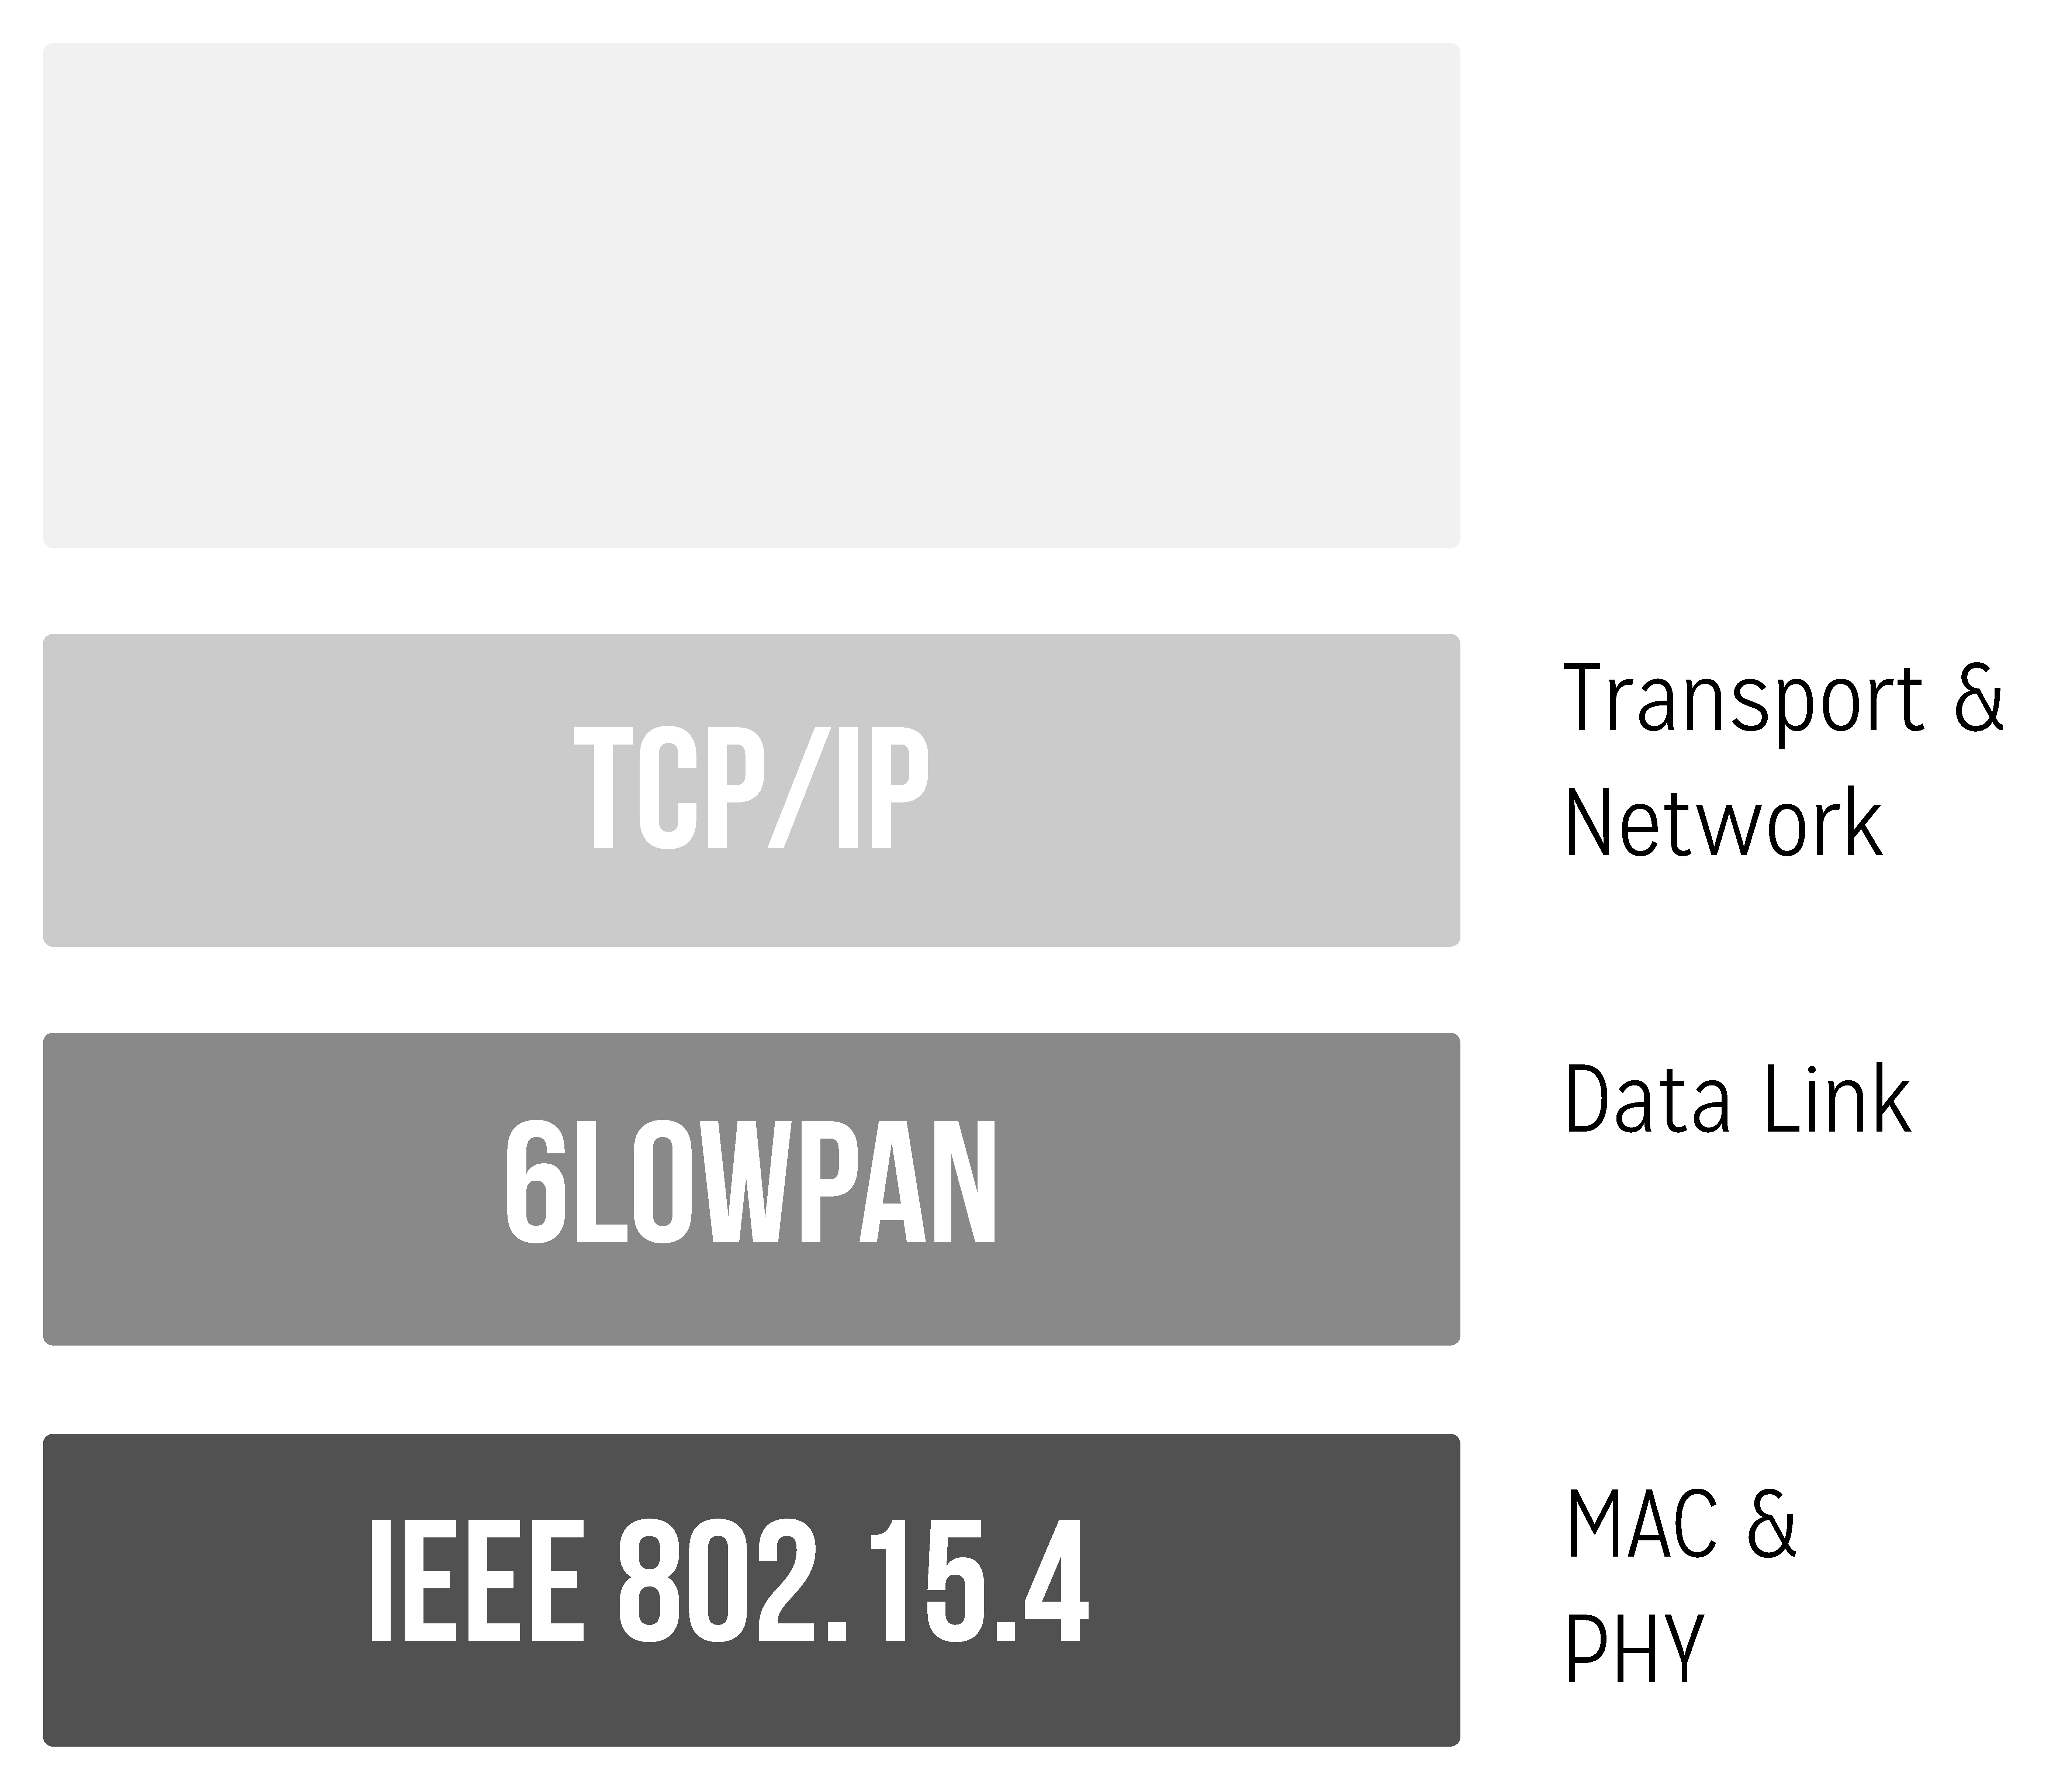
\includegraphics[width=0.9\textwidth]{graphics/networkstack.eps}
  \caption{Comparison of traditional and IoT Network Stacks.}
  \label{fig:networkstack}
\end{figure}

Because the IoT differs from the ``traditional'' Internet in crucial aspects, the use of a custom network stack as illustrated in Fig. \ref{fig:networkstack} is necessary.\\
The IEEE 802.15.4 Data Link and Physical layers have been optimized for energy-efficiency and the ability to be deployed on cheap device. Its \gls{MTU} is a mere 127 bytes. This limitation conflicts with the minimal MTU of 1280 bytes dictated by IPv6, generating the demand for an adaptation layer: 6LoWPAN. Here, IPv6 headers are compressed; packets exceeding the new 127 byte MTU are fragmented. The fragments produced can be reassembled by all border routers connecting a 6LoWPAN network to the Internet.

\subsection{Requirements and key challenges for routing protocols}
\label{subsec:intro_requirements}
%==============================================================================
\cite{RFC-5826}, \cite{RFC5548} and \cite{RFC5867} list requirements for a routing protocol in the differing scenarios of Home Automation, Urban-\glspl{LLN} or Building Automation. Even though these fields may all be categorized as IoT-adjacent, their characteristics differ vastly in terms of traffic flow and patterns, network size, and degree of mobility. %(TODO. lieber nochmal überprüfen)
Despite these differences, the domains of their requirements can be classified into four categories:

\begin{description}
\item{\emph{Traffic Patterns:}} A routing protocol for the IoT has to match the traffic pattern of its area of deployment. Since patterns vary from network to network, as shown in \ref{subsec:intro_IoT}, there is most likely not \emph{one} protocol to rule them all, but rather at least one appropriate protocol for each subdivision of IoT deployments.

\item{\emph{Energy efficiency:}} The deployment of battery-driven nodes running autonomously for extended periods of time is one of the cornerstones of the IoT. A routing protocol that is resourceful in terms of energy consumption is vital to the functionality of an IoT-based network.
Closely tied to these efforts is the topic of energy-\emph{awareness}. A protocol able to communicate its nodes' constraints is able to make more informed routing decisions based on this information.

\item{\emph{Scalability:}} The protocol should scale to a network size ranging from 100 to 1,000,000 nodes, both in terms of performance as well as memory usage: an increase in network size may not lead to an explosion in routing table size.

\item{\emph{Mobility:}} Even though the \gls{IoT} does not typically experience a lot of movement, a suitable routing protocol should be able to cope with sparse location changes of single nodes.
\end{description}
% TODO: was ist mit code image size?
% challenges
In addition to the requirements listed above, the nature of the \gls{IoT} poses unique challenges to any routing protocol serving them.

\begin{description}
\item{\emph{Bidirectionality:}} As with all wireless networks, bidirectional connectivity between links is not guaranteed. %Even moreso in \gls{IoT} deployments:
A routing protocol for the \gls{IoT} has to be able to recognize and avoid unidirectional links at the least, and may be able to use them in one direction at best.

\item{\emph{Transmitter usage:}} Concerning energy consumption, the transmitter is the most expensive component of a constrained device.
It is therefor advisable to use it as sparsely as possible. %, letting the device go into deep sleep mode when it is not needed. % TODO: was ist mit wakeup costs?
\end{description}

\subsection{Related research}
\label{subsec:intro_related_fields}
%==============================================================================
Because the \gls{IoT} is a budding field, few research is explicitly tailored to its characteristics.
Nonetheless, adjacent fields have produced work which explores problems which are familiar to the \gls{IoT}, most notably the research fields of \glspl{MANET}, \glspl{DTN} and \glspl{LLN}.